In this section the results will be shown for this project.

\subsection{OpenMP}
\label{sec:openmp}
As mentioned in [ref to tools] OpenMP can be used to parallelize loops and other easy functions that can be easy to make parallel. Figure \ref{fig:graph_generation} shows a graph of the amount of time spent generating the graph as a function of the amount of cores that were assigned to the program. The figure shows that the time spent is  dependent on the amount of CPUs. Each time the amount of CPUs doubles the time spent is halved. 
 % These experiments have been on the DAS with validation on.

\begin{figure}[!h]
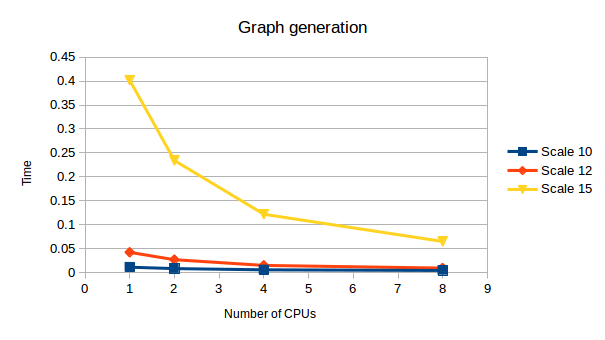
\includegraphics[width=\textwidth]{images/openmp_graphgeneration.png}
\caption{This graphs shows the graph generation time as a function of the number of CPUs used by the program}
\label{fig:graph_generation}
\end{figure}


In figure \ref{fig:openmp_scale_cpu} the TEPS can be see as a function of the CPUs used on the left and the scale on the right. Both graphs show that the amount of lines that can be traversed is almost constant.

\begin{figure}[!h]
\centering
\begin{subfigure}{.5\textwidth}
  \centering
  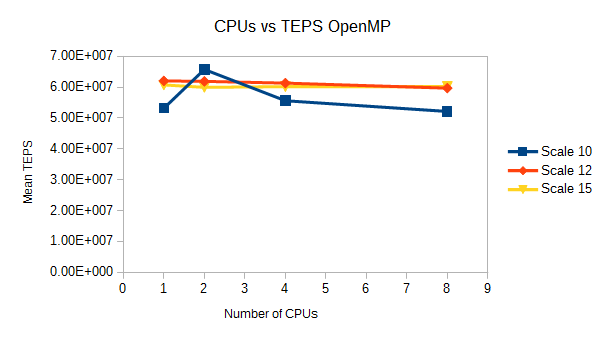
\includegraphics[width=\linewidth]{images/openmp_cpus.png}
  %\caption{A subfigure}
  %\label{fig:sub1}
\end{subfigure}%
\begin{subfigure}{.5\textwidth}
  \centering
  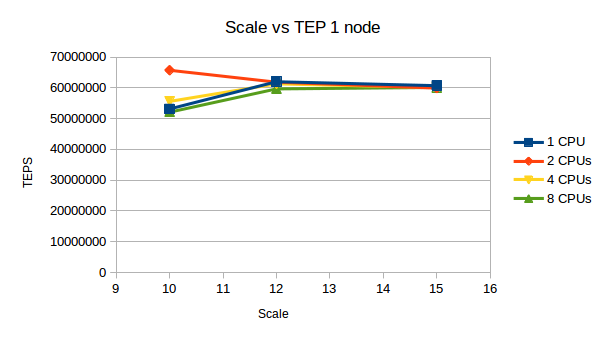
\includegraphics[width=\linewidth]{images/openmp_scale.png}
  %\caption{}
  %\label{fig:sub2}
\end{subfigure}
\caption{These figures show the effect of different of scale and the number of CPUs on the TEPS}
\label{fig:openmp_scale_cpu}
\end{figure}

\subsection{DAS-4}
In this section the results are shown of using the \texttt{graph500\_mpi\_simple} on the DAS-4. As mentioned in section[methodology], when the program is run for scales larger than 15 the program freezes. Only experiments done in next section and in section \ref{sec:openmp} have been done with validation, all other experiments have been done without.

\subsubsection{Turning validation off}
\label{sec:noval}
 Figure \ref{fig:val_vs_noval} shows the results of the amount of TEPS against the scale and the number of nodes. The figures shows that there is a difference in the number of TEPS with and without the validation. The difference can be up to 150\% in the case of scale 15 with 16 nodes. What can be noticed in figure \ref{fig:nodes_val_noval} is that the same trends are followed as the number of nodes increases. Another thing, which can be seen in figure \ref{fig:scale_val_noval}, is that the ratio of TEPS increase as the scale increases.
\begin{figure}[!h]
\centering
\begin{subfigure}{.5\textwidth}
  \centering
  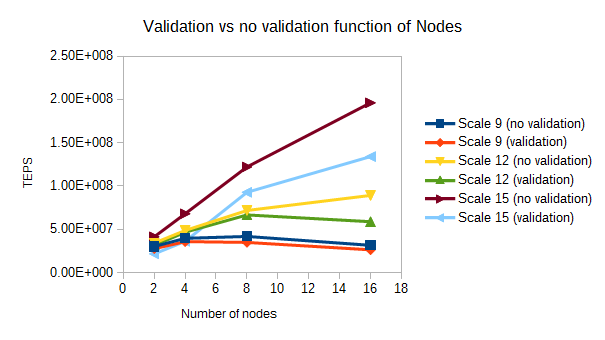
\includegraphics[width=\linewidth]{images/nodes_scale_vs_noscale.png}
  \caption{As a function of nodes}
  \label{fig:nodes_val_noval}
\end{subfigure}%
\begin{subfigure}{.5\textwidth}
  \centering
  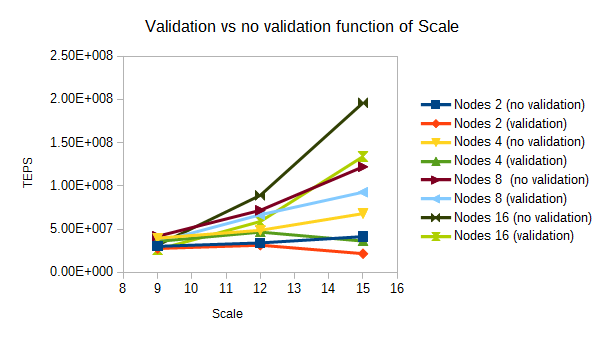
\includegraphics[width=\linewidth]{images/scale_val_vs_noval.png}
  \caption{As a function of scale}
  \label{fig:scale_val_noval}
\end{subfigure}
\caption{These figures show the effect of different of scale and the number of CPUs on the TEPS between the program with and without validation.}
\label{fig:val_vs_noval}
\end{figure}



\subsubsection{Nodes and Scale}
\label{res:nodes_scale}
In figure \ref{fig:das_no_val} shows the amount of TEPS increases as the number with the number of nodes. The larger the amount of nodes the more edges can be traversed, as seen in figure \ref{fig:scale_no_val}. This increase in TEPS can be seen up til a certain point. After this point the amount of TEPS decreases again. This tipping point can be seen in a any of the line except for the smaller scales in which the line is close to constant for any scale.
Figure \ref{fig:nodes_no_val} shows the same data but then as a function of the number of nodes. What can be seen in these figures is that the amount TEPS increases as the nodes increases per scale. These are fairly straight lines. The thing to notice is that scale 21 is performs the best of each investigate number of nodes, although for 2 and 4 nodes the amount of TEPS always about the same, independent of the scale of the problem.
One interesting thing to note is that the measurements done on scale 30 have less TEPS than the TEPS for scale 15.

\begin{figure}[!h]
\centering
\begin{subfigure}{.5\textwidth}
  \centering
  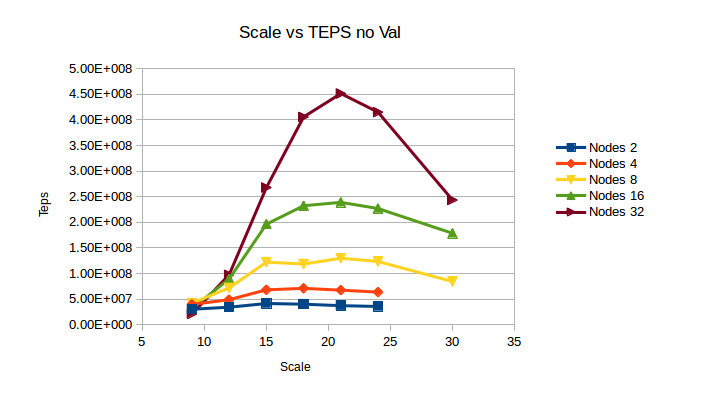
\includegraphics[width=\linewidth]{images/nodes_no_val.png}
  \caption{TEPS as a function of nodes for different scales.}
  \label{fig:nodes_no_val}
\end{subfigure}%
\begin{subfigure}{.5\textwidth}
  \centering
  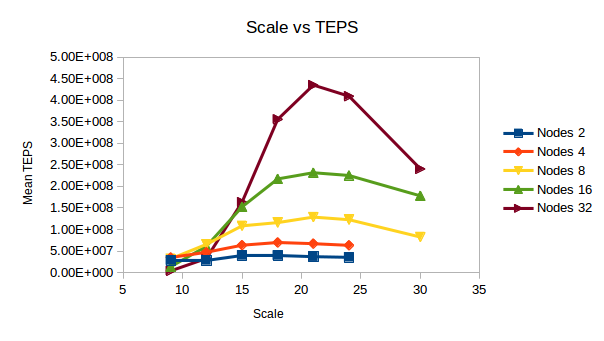
\includegraphics[width=\linewidth]{images/scale_no_val.png}
  \caption{TEPS as a function of scale for different amount of nodes.}
  \label{fig:scale_no_val}
\end{subfigure}
\caption{This figure shows the change in the amount of TEPS as a function of scale and nodes.}
\label{fig:das_no_val}
\end{figure}

\subsubsection{No InfiniBand}
The experiments on the DAS-4 have also been done run without InfiniBand. The results are similar to what has been seen previously. As before figure \ref{fig:scale_no_infini} shows an increase in TEPS as the scale increases till a certain tipping point, but unlike what has been seen in figure \ref{fig:scale_no_val} the tipping point has not been yet been reached at scale 24. Figure \ref{fig:scale_no_infini} shows that slope between scale 21 and 24 is very small, but not yet reached. The difference between the maximum value for 16 nodes from the results of section \ref{res:nodes_scale} is 6 times as large as the maximum value for the same amount of nodes from the InfiniBand experiments.
Figure \ref{fig:scale_no_infini} also shows the same trends as figure \ref{fig:scale_no_val}. 
 
\begin{figure}[!h]
\centering
\begin{subfigure}{.5\textwidth}
  \centering
  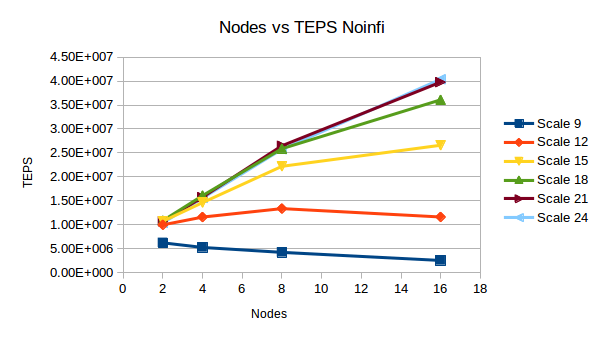
\includegraphics[width=\linewidth]{images/nodes_no_infini.png}
  \caption{TEPS as a function of nodes for different scales.}
  \label{fig:nodes_no_infini}
\end{subfigure}%
\begin{subfigure}{.5\textwidth}
  \centering
  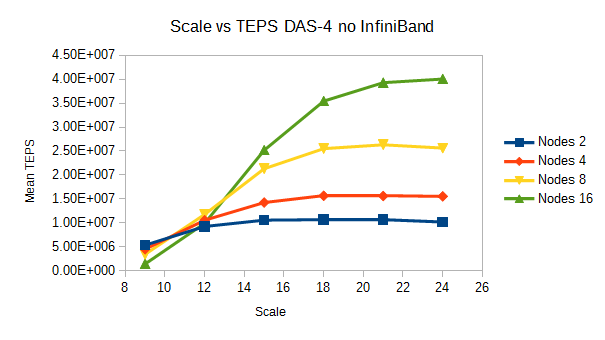
\includegraphics[width=\linewidth]{images/scale_no_infini.png}
  \caption{TEPS as a function of scale for different amount of nodes.}
  \label{fig:scale_no_infini}
\end{subfigure}
\caption{This figure shows the change in the amount of TEPS as a function of scale and nodes on the DAS-4 without using InfiniBand.}
\label{fig:das_no_infini}
\end{figure}

\subsection{OpenNebula}
The OpenNebula results can best be compared the results on the DAS-4 without InfiniBand, because the VMs on the OpenNebula also do not use Infiniband.
Looking at figure \ref{fig:das_opennebula} it is clear to see that graph is far less clear. IN both graphs you can see far more intersections and results are far less smooth than the other than the previous two graphs(figure \ref{fig:das_no_val} and \ref{fig:das_no_infini}). The difference between using 4 and 8 nodes is much less clear on the OpenNebula, four nodes sometimes has an even better performance than eight nodes.
As a whole the trends can be seen only again a few factors smaller than the results of the DAS with infiniband turned off.

\begin{figure}[!h]
\centering
\begin{subfigure}{.5\textwidth}
  \centering
  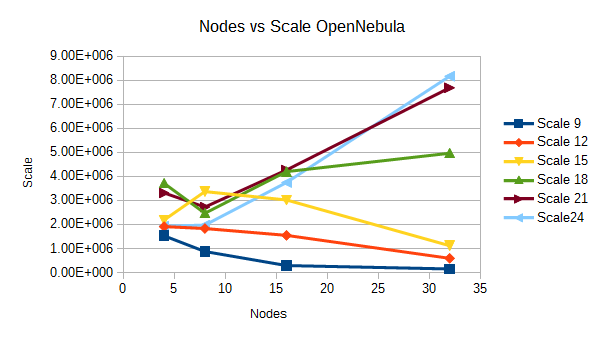
\includegraphics[width=\linewidth]{images/nodes_opennebula.png}
  \caption{TEPS as a function of nodes for different scales.}
  \label{fig:nodes_opennebula}
\end{subfigure}%
\begin{subfigure}{.5\textwidth}
  \centering
  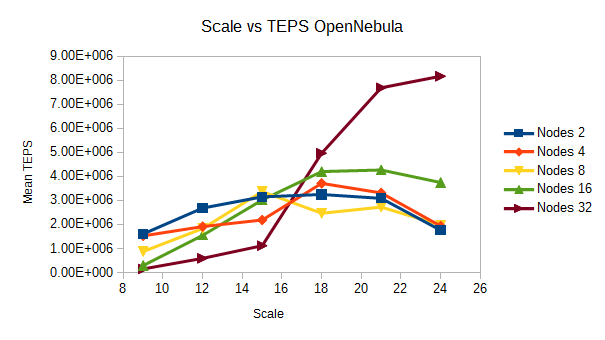
\includegraphics[width=\linewidth]{images/scale_opennebula.png}
  \caption{TEPS as a function of scale for different amount of nodes.}
  \label{fig:scale_opennebula}
\end{subfigure}
\caption{This figure shows the TEPS vs the scale and nodes for the experiments done on OpenNebula of the DAS-4.}
\label{fig:das_opennebula}
\end{figure}

\subsection{Communication}
In this section the results are shown with respect to the communication between the nodes.
\subsubsection{IMB benchmark}
On each of the systems the IMB benchmark has been done. To find the time it takes to send messages between to machines. The times which are relevant are 0, 1028 and 2048 bytes. The 0 bytes times shows the time it takes to send the finished message, 1028 bytes gives an indication of how much time it will take to send a message without a completely full buffer, and lastly the 2048 shows the time it takes to send a full buffer. The complete table is shown in Appendix [REF to appendix].
\begin{table}[!h]
\begin{tabular}{|l|l|l|l|}
\hline
Bytes & DAS-4 ($\mu sec$) & DAS-4 no InfiniBand($\mu sec$) & OpenNebula ($\mu sec$)\\ \hline
0 & 3.81 &  46.55  & 112.75  \\ \hline
1024 & 4.93 & 56.97  &  130.76 \\ \hline 
2048 & 269.74 & 5.96 & 68.36 \\ \hline
\end{tabular}
\caption{This figure shows the IMB benchmarks on the different platforms used. All times are an average of a 1000 messages sent. Only the relevant sizes have been shown.}
\label{tab:imb_bench}
\end{table}

\subsubsection{Message count}
The message count is an important number for calculate the communication time. The amount of data which is sent per message is known, but the number of messages is not known. As mentioned before in the paper by Suzumaru\cite{suzumura2011performance} an estimation for the amount of bytes which is, see equation \ref{eq:communication_size}. In figure \ref{fig:das_scale_messages} two plot can be seen. The figure shows that the estimation of data send is correct and with this the number of messages can derived by using this estimation. There is one thing to notice is that there is a factor two difference between the number of messages. 
\begin{figure}[!h]
\centering
\begin{subfigure}{.5\textwidth}
  \centering
  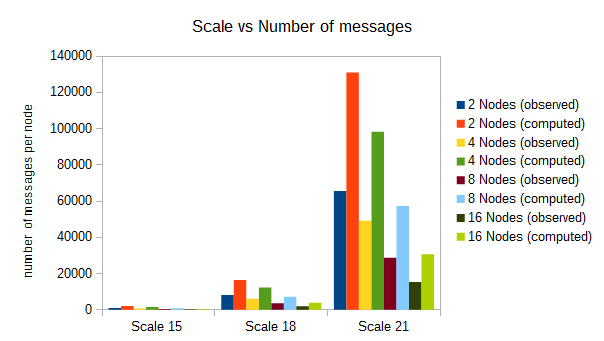
\includegraphics[width=\linewidth]{images/scale_vs_messages.png}
  \caption{The number of messages as a function of scale for different number of nodes.}
  \label{fig:scale_messages}
\end{subfigure}%
\begin{subfigure}{.5\textwidth}
  \centering
  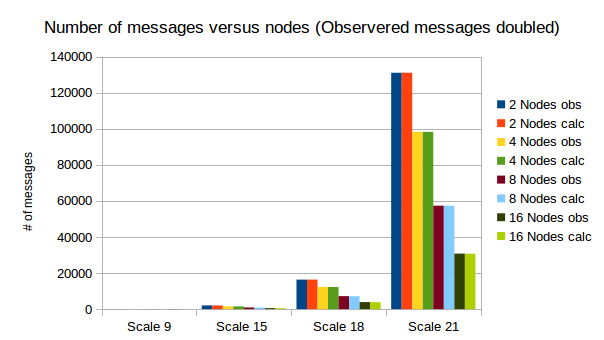
\includegraphics[width=\linewidth]{images/scale_vs_messages_doubled.png}
  \caption{The same graph as figure \ref{fig:scale_messages}, but with the observed number of messages doubled}
  \label{fig:scale_messages_doubled}
\end{subfigure}
\caption{This figure shows how the number of messages grows for 4 different scales and 2 to 16 nodes. The observed number is the number of messages sent when the buffer is full + the messages send with left overs, see section \ref{med:comm}}
\label{fig:das_scale_messages}
\end{figure}

\subsection{The model}
